\documentclass[10pt,a4paper]{article}
\usepackage[utf8]{inputenc}
\usepackage{amsmath}
\usepackage{amsfonts}
\usepackage{amssymb}
\usepackage{graphicx}
\usepackage[margin=1in]{geometry}
\usepackage{multicol}
\usepackage{tabularx}
\usepackage{caption}
\mathchardef\mhyphen="2D
\usepackage{enumitem}
\newlist{myitems}{enumerate}{1}
\setlist[myitems]{label=[\arabic*], font=\bfseries, resume}
\usepackage{lipsum}
\usepackage{color}
\usepackage{subcaption}
\usepackage{algorithm}
\usepackage[noend]{algpseudocode}
\usepackage{tabto}
\usepackage{rotating}
\usepackage{tikz}
\usepackage{wrapfig}

\newsavebox{\fmbox}
\newenvironment{fmpage}[1]
{\begin{lrbox}{\fmbox}\begin{minipage}{#1}}
{\end{minipage}\end{lrbox}\fbox{\usebox{\fmbox}}}


\makeatletter
\def\BState{\State\hskip-\ALG@thistlm}
\makeatother


\begin{document}
%\textmd 
\vspace{5mm}
\begin{flushleft}
{\LARGE \textbf{Measuring rotation invariance in
pre-trained multi-layer perceptrons}}\\
\vspace{10mm}
{\small \textbf{Claudia Winklmayr\\ 
\textit{Bernstein Center for Computational Neuroscience Berlin}\\
Supervision: Prof. Klaus Obermayer, Youssef Kashef\\
\textit{Neural Information Processing Group, TU Berlin}
}}
\vspace{5mm}
\end{flushleft}

\begin{abstract}
\noindent In this project we initialized a Multilayer Perceptron (MLP) with parameters from an Autoencoder (AE) trained to reconstruct rotated images of the MNIST dataset. We evaluated the MLP's classification performance, and studied whether the network would arrive at a rotation-invariant representation of the inputs and in which way information about the rotation would be conserved. We found that on the one hand activity patterns elicited by images of different rotation degrees become more similar in higher layers of the network. On the other, hand neurons which contribute strongly to classification remain sensitive to rotation.
\end{abstract}

\section{Introduction}

Artificial neural networks achieve impressive results in processing and classifying visual data but the underlying processes still remain poorly understood, especially we lack understanding of how the visual data is represented within the network. Ideally such a representation should be robust to variations caused e.g. by (small amounts of) noise, scaling or rotation. A robust (or \textit{invariant}) representation is also plausible from a biological standpoint since real-world visual input is prone to variability, yet humans and animals are able to classify it reliably. In artificial neural networks invariance can be achieved by mapping the input onto prototypes which are subsequently classified. A network capable of this strategy was proposed by \cite{Olshausen}. 
\newline

\noindent Although finding invariant prototypes of the input classes is a feasible strategy, it is not clear whether this strategy is pursued by a given neural network. 
One approach to simplifying training and increase robustness to input variation is to use parameters from a different network which already learned a related task. Such a policy was successfully applied for example in \cite{Benigo}\newline
Here we used this approach and initialize classifier networks with parameters from autoencoders which were previously trained to reconstruct rotated images. From the nature of the reconstruction task, we hypothesized the network would find some rotation-invariant representation of the input as well as information about the rotation itself. The main question we ask is how the information about the input's rotation is represented in the network and whether it can be separated from information about the input's class. 


\section{Setup}
For the classification task we used two Multilayer Perceptrons (MLP) with four fully connected layers of decreasing size and a final Softmax layer for classification. All weights connecting the first four layers were taken from trained autoencoders (AEs) and left unchanged. Only the set of weights connecting the fourth layer to the Softmax classifier were trained by gradient decent.



\subsection{Pretraining the weights}

%----------------Begin Figure--------------------%
\begin{figure}[h]
\centering
\begin{subfigure}{.5\textwidth}
  \centering
  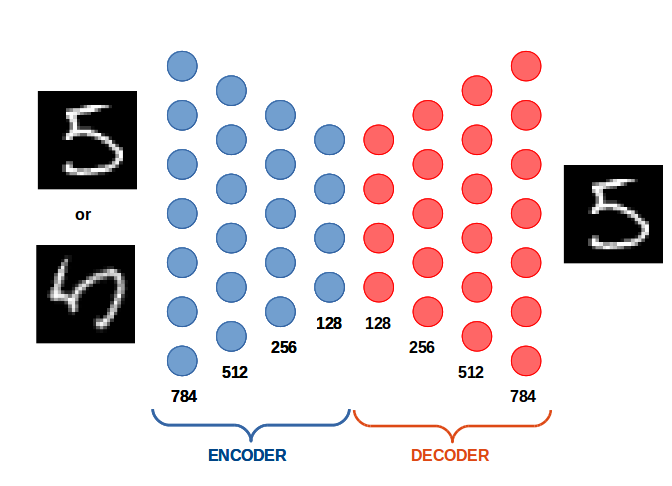
\includegraphics[width=.8\linewidth]{enc_dec_mnist.png}
  \caption{\footnotesize{Autoencoder (AE)}}
  \label{fig:AE}
\end{subfigure}%
\begin{subfigure}{.5\textwidth}
  \centering
  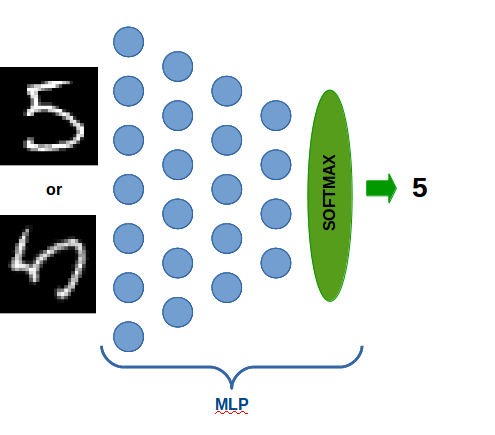
\includegraphics[width=.65\linewidth]{mlp_mnist.png}
  \caption{\footnotesize{Multilayer perceptron (MLP) from AE}}
  \label{fig:MLP}
\end{subfigure}
\caption{\footnotesize{Schematic illustration of the AE and MLP setup.}}
\label{fig:AE_and_MLP}
\end{figure}
%------------------End Figure--------------------%

\noindent As depicted in Figure \ref{fig:AE}, the AEs have a bottleneck architecture with decreasing size of encoder layers (784, 512, 256 and 128 neurons respectively) and correspondingly increasing sizes of decoder layers. In the following we will refer to the number of neurons in a specific layer as $N^{layer}$ (e.g. $N^1 = 784$). The bottleneck setup guarantees that the network learns a representation of the input that is different from the identity. During training the vector of decoder weights $W_{dec}$ was enforced to be the transpose of the the encoder weight vector $W_{enc}$, i.e. $W_{dec} = W_{enc}^T$. 
The AEs are trained using backpropagation of cross-entropy loss
        \begin{displaymath}
        E = \frac{1}{N}\sum_{n=1}^{N}[p_n log(\hat{p}_n) + (1 - p_n)log(1 - \hat{p}_n)]
        \end{displaymath}
        
\noindent with sigmoid-nonlinearity 
		\begin{displaymath}
		\hat{p}_n  = (1 + \exp(-x))^{- 1}.
		\end{displaymath}
where $p_n$ are the class probabilities and $N$ is the number of samples.   Training using minibatch gradient descent (batch size of 1000) lasted for 380,000 iterations. The learning rate was set to 0.01 and reduced stepwise every 10,000 iterations by $10\%$.
The momentum was set to 0.9 and weight decay to 0.004 (for a detailed description of the training procedure see \cite{Oliver}).


\subsection{Building the MLP}
To understand how different strategies of training the AE affect the classification performance of the MLP, we built two MLPs: the first one used $W_{enc}$ of an AE trained with the normal MNIST set (AEUR); the second one uses weights of an AE trained with MNIST samples that were rotated by a randomly chosen angle $\phi \in \{-90, -75, -60, \dots, 0, \dots,  90\}$ (AER).\footnote{Both autoencoders are trained to reconstruct the unrotated MNST set.}
The $W_{enc}$ is kept constant and a Softmax classifier is attached on top of the fourth encoder layer. Each of the 10 neurons in the Softmax layer codes for one of the 10 digit-classes. In both cases the weights connecting the encoder to the Softmax layer are trained with batch gradient decent using the unrotated MNIST training set (100,000 images), 1000 iterations, a batch size of 128 and constant learning rate of $\lambda = 0.05$. We distinguish the two resulting MLPs by the labels of the corresponding AEs (AER and AEUR).
\newline As will be apparent in the following results, training only the final layer for classification leads to an overall low accuracy of the MLPs (around 80\% in the best case). This can easily be overcome by fine-tuning the whole network after training the Softmax layer. However, our goal was not to achieve the highest possible classification accuracy but to study how the network learns to interpret rotated images. Fine-tuning for better classification might lead to loss of rotation information.


\subsection{Datasets}

\noindent All of the following results were computed using different variants of the MNIST test set (10,000 images of handwritten digits, 28$\times$28 pixels each). By MNIST or MNIST$_{0}$ we mean the original (unaltered) set of images. MNIST$_{mix}$ refers to a manipulated version of this set, where each image is rotated by a randomly chosen angle $\phi \in \{-90, -75, -60, \dots, 0, \dots,  90\}$. This corresponds to the version of MNIST with which the AER auto encoder was trained. \newline
\noindent When studying the behavior of the classifier at specific rotation angles we will rotate the whole test set by this angle and indicate the rotation angel by subscript (e.g. MNIST$_{30}$ or MNIST$_{-30}$). 
If we want to look at the behavior of the network for specific digits (e.g. how well the network classifies the digit $7$ depending on different degrees of rotation) we will indicate the respective digit by superscript: e.g. MNIST$_{30}^{7}$ means the dataset that contains only images of the digit $7$, all rotated by 30 degrees.


\section{Performance Comparison}

\noindent In this section we will compare the performance of a classifier trained only with the standard MNIST dataset (AEUR) to the performance of a classifier trained with different rotations (AER). \newline
The first thing to observe is that, while both classifiers perform nearly equally on the unrotated set, AER obviously outperforms AEUR on any rotated set (see Figure \ref{fig:AERvsAEUR_angles}). Also noteworthy is the low accuracy of both networks even on the original dataset (a little over 80 \% in the best case as compared to nearly 100\% as can be achieved even with less complex MLPs). This is mostly due to the fact that for classification we only trained the final layer. 


%----------------Begin Figure--------------------%
\begin{wrapfigure}[11]{R}{0.5\textwidth}
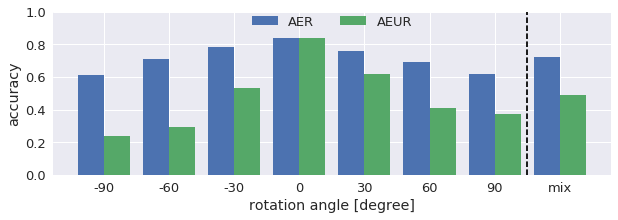
\includegraphics[width=\linewidth]{AERvsAEUR_angles.png}
\captionof{figure}{\footnotesize{Comparison of AER (blue) and AEUR (green) on datasets with different rotation angles (see section 1).}}
  \label{fig:AERvsAEUR_angles}
\end{wrapfigure}
%------------------End Figure--------------------%


%----------------Begin Figure--------------------%
\begin{figure}[b!]
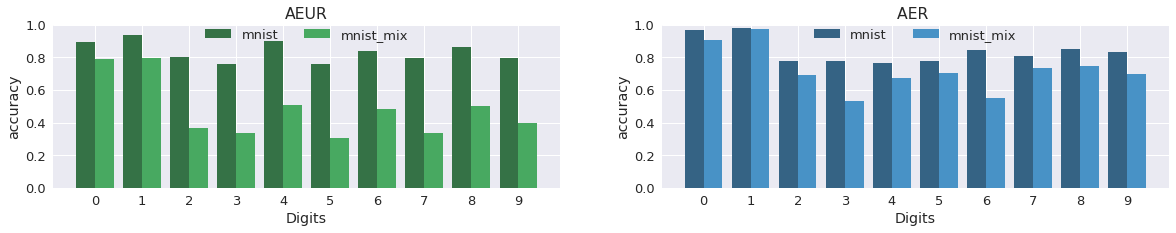
\includegraphics[width=1\textwidth]{AER_AEUR_digits.png}
\caption{\footnotesize{\footnotesize{Comparison of AER and AEUR for different digits (rotated and unrotated).}}}
\label{fig:Digits}
\end{figure}
%------------------End Figure--------------------%

\noindent It is important to note that classification accuracy is not the same across digits and also rotation affects some digits more than others. Figure \ref{fig:Digits} shows how the classification accuracy of the two networks varies for MNIST$_{0}^{i}$ vs. MNIST$_{mix}^i$ for $i \in 0 \dots 9$.\newline 

\noindent Whereas for AEUR we see massive drops in performance as we move from MNIST$_0$ set to MNIST$_{mix}$, the behavior of AER is more robust. Especially for digits with 'simple' shapes like 0, 1 and 7, we see only very little change in performance, hinting at rotation-invariant representations of those numbers.

\subsection{Spike Triggered Average}
To understand the behavior of the two networks we look at which inputs elicit high responses of the Softmax neurons. Figure \ref{fig:STA_Softmax} shows a version of spike triggered average (STA)\footnote{Spike Triggered Average (STA) is a measure from neuroscience used to characterize the response properties of a neuron by calculating the average over all inputs that triggered an action potential. In artificial neural networks using sigmoid non-linearities one usually considers all inputs, weighted by the activation they caused in a given unit. The interpretation of our final Softmax layer, however, is more similar to that of a biological neuron, since only the most active neuron is relevant for classification. Therefore we don't calculate the weighted average over all inputs but only over those which caused a given neuron to be the most active in the Softmax layer.} for AEUR(a) and AER(b) for all 10 Softmax neurons (columns) and several datasets (rows). To generate the images we classified 5000 images (i.e.$\approx$500 per digit type). Whenever one of the ten Softmax neurons was the most active we added the image that caused this activity to this neuron's STA-image. Comparing AER and AEUR in Figure \ref{fig:STA_Softmax} it becomes clear that as the rotation angle increases the images created with AEUR become more and more blurry until at a rotation angle of 90 degrees some digits are not even recognizable, again AER shows a much more stable representation of the data. 

%----------------Begin Figure--------------------%
\begin{figure}[h]
\centering
\begin{subfigure}{.49\textwidth}
  \centering
  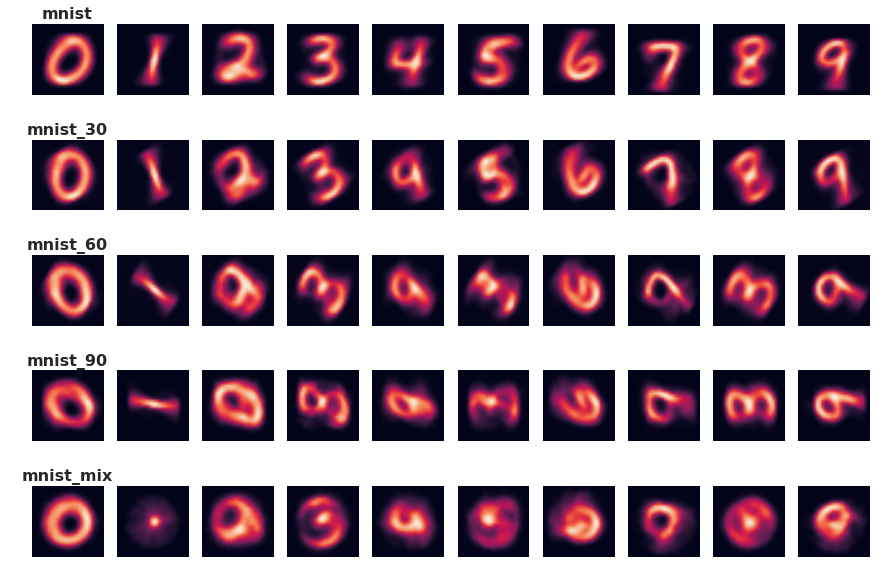
\includegraphics[width=1\linewidth]{STA_Softmax_AEUR_new.png}
  \caption{\footnotesize{AEUR}}
  \label{fig:STA_AEUR}
\end{subfigure}%
\begin{subfigure}{.49\textwidth}
  \centering
  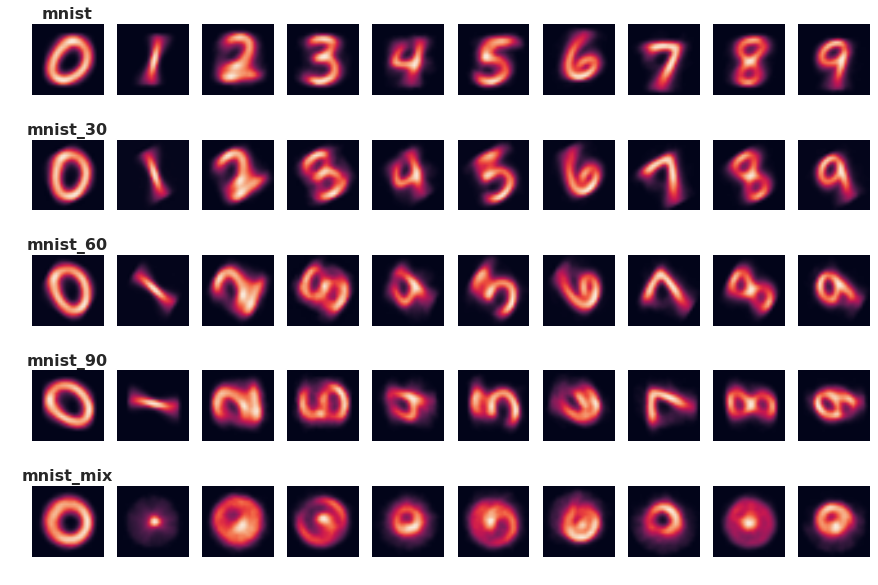
\includegraphics[width=1\linewidth]{STA_Softmax_AER_new.png}
  \caption{\footnotesize{AER} }
  \label{fig:STA_AER}
\end{subfigure}
\caption{\footnotesize{Average of images that caused a Softmax neuron to be the most active of the layer. The columns contain the resulting images for each Softmax neuron in networks AEUR (left) and AER (right). The rows correspond to different datasets starting with the unperturbed MNIST set in the top row, going through rotation angles 30, 60 and 90 degrees and the MNIST$_{mix}$ in the bottom line.}}
\label{fig:STA_Softmax}
\end{figure}

%------------------End Figure--------------------%



\section{Layer Comparison}
To compare how the first four layers of the AER-MLP (without  Softmax) differ in their behavior with respect to the rotation of the inputs, we will focus on six different datasets:  $\mathcal{D} = \{$ MNIST, MNIST$_{mix}$, MNIST$_{-60}$, MNIST$_{-30}$, MNIST$_{30}$, MNIST$_{60}$ $\}$. The last four sets were selected to investigate the behavior of single angle rotations as well as to compare orthogonal pairs, i.e $-60 \deg$ vs. $30\deg$ and $-30\deg$ vs. $60\deg$. 

\subsection{General}
%----------------Begin Figure--------------------%
\begin{figure}
\centering
\begin{subfigure}{.5\textwidth}
  \centering
  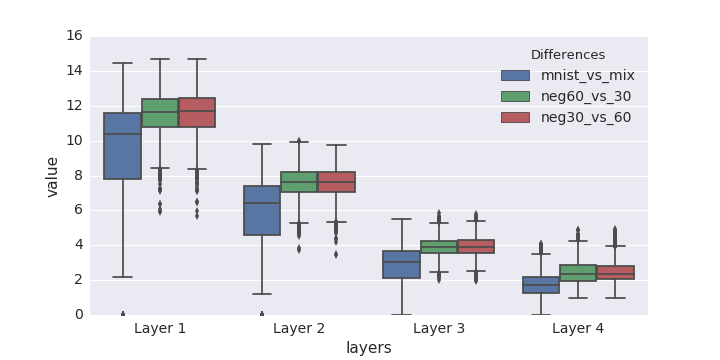
\includegraphics[width=1\linewidth]{euc_diffs.png}
  \caption{\footnotesize{Averaged Euclidian distances}}
  \label{fig:euc_dists}
\end{subfigure}%
\begin{subfigure}{.5\textwidth}
  \centering
  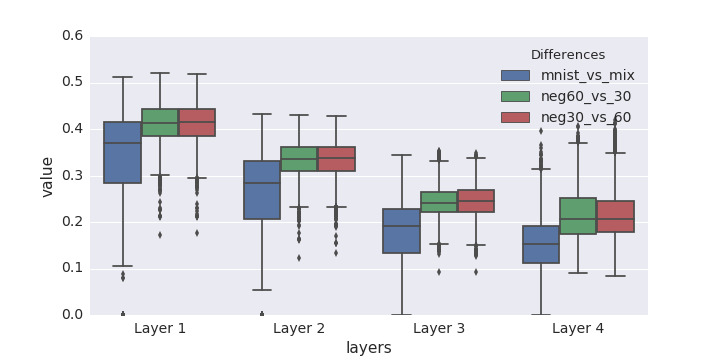
\includegraphics[width=1\linewidth]{euc_diffs_normalized.png}
  \caption{\footnotesize{Averaged Euclidian distances normalized by number of neurons per layer}}
  \label{fig:euc_dists_normalized}
\end{subfigure}
\caption{\footnotesize{Boxplot of Euclidian distances between the layers' activity vectors for three pairs of datasets: MNIST vs. MNIST$_{mix}$ (blue), 30 vs. -60 degree (green) and 60 vs. -30 degree (red). In both figures we see the average distances decrease as we go further in the network. }}
\label{fig:Euclidian_distances}
\end{figure}
%------------------End  Figure--------------------%}


In the first step we compare the layer-wise patterns of activity elicited by the different degrees of input rotation. To this end we separate the datasets into 3 pairs:  no rotation vs. mixed rotation, 30 vs. -60 degree and 60 vs. -30 degree. For each pair we then present the network with samples from both datasets, interpret the activation of neurons in a given layer as a vector in $\mathbb{R}^{N^{layer}}$, and compute the Euclidian distance between these vectors for each sample. This yields a measure of how the same image causes different activations depending on its rotation. Figure \ref{fig:Euclidian_distances}  shows these distances averaged over all samples. \newline 

\noindent It is apparent that as the number of layers increases, the patterns become increasingly similar for the two orthogonal pairs as well as for the comparison between the unrotated data and the set of mixed rotations. This indicates that the representation of the input as a pattern of layer activities becomes less sensitive to rotation further inside the network. This behavior can still be observed if we account for the different numbers of neurons in the layers: the boxplots in Figure \ref{fig:euc_dists_normalized} show the same Euclidian distances, scaled by $1 / \sqrt{N^{layer}}$.
\footnote{The resulting measure can be thought of as a fraction of the 'maximal possible distance per layer'. For example, in layer 1 there are 784 neurons each having a value between 0 and 1. The maximum distance, therefore, is $\sqrt{784}$. A value of 1 in \ref{fig:euc_dists_normalized} would correspond to this maximal distance.}


\subsection{Most Active Neurons}

\noindent Since the activation functions of our networks are sigmoids with values between 0 and 1, we assume that neurons having an active part in classification should express high values of activity, i.e. values close to 1. In this section we therefore identify the most active neurons in each layer and study how their activity depends on the rotation and class of the input. \newline

\noindent To determine the most active neurons for a given layer and dataset, we present the network with samples from this dataset and save, for each sample, the IDs of the most active 10\% of neurons. We then count how often each neuron of the selected layer was among the layer's most active ones, and normalize the result by the total number of inputs, to yield a probability value $p_{10}(n)$.\newline

\noindent Figure \ref{fig:MostActive_2} shows the values of $p_{10}(n) $ for the first 80 neurons in layer 2. (For a view of the entire network see Figure \ref{fig:MostActive_all}). Throughout all layers the patterns for different datasets show very strong overlap,  indicating that classification is always driven by the same neurons, independent of the rotation of the input image. We take this to mean that there are no single \textit{rotation neurons} coding for the degree of rotation independent of the class of inputs. 


\subsection{Three types of neurons}

%------------------Begin Figure--------------------%
\begin{figure}[t!]
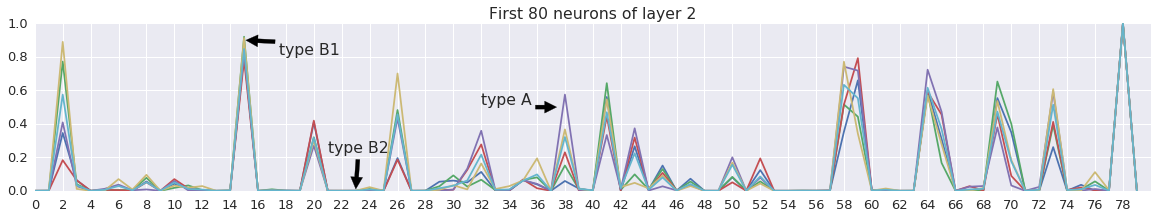
\includegraphics[width=1\textwidth]{MostActive_Layer2_cut.png}
\caption{\footnotesize{Values of $p_{10}(n)$ for the first 80 neurons in layer 2. The line colors mark different datasets from $\mathcal{D}$. The strong overlap indicates that the IDs of neurons playing an active role in classification do not vary much across datasets. The black arrows point to examples of Type A, B1 and B2 neurons which are distinguished by the variance of $p_{10}(n)$ with respect to the datasets (see section 4.3).}}
\label{fig:MostActive_2}
\end{figure}
%------------------End Figure--------------------%

\noindent Looking at Figure \ref{fig:MostActive_2}, we find that although the IDs of the most active neurons do not change with the datasets, the value of $p_{10}(n)$ nevertheless seems to be tied to the degree of input rotation. From this observation we go on to define two main types of neurons, depending on the variance of $p_{10}(n)$ with respect to the datasets: \textit{Type A} neurons, for which $p_{10}(n)$ varies strongly with input rotation and \textit{Type B} neurons for with  $p_{10}(n)$ shows little variation. We then further divide the group of Type B neurons into those that show high values of $p_{10}(n) $ (Type B1) and those for which the values of $p_{10}(n)$ are low (Type B2). Examples for all three kinds of neurons are marked in Figure \ref{fig:MostActive_2}.\newline

\noindent  More formally, we find the neurons of each type (in a given layer) by the following procedure: first calculate $p_{10}^{l}(n | d)$, i.e the probability of the neuron $n$ to be among the 10\% of most active neurons in layer $l$ when presented with a sample from dataset $d$. To simplify the following expressions we will assume to always stay in one layer and omit the $l$ superscript. Then we calculate the mean of $p_{10}(n | d)$ over all datasets, i.e. $\mu_{10}(n) = \frac{1}{|\mathcal{D}|} \sum_{d \in \mathcal{D}} p_{10}(n|d)$, and the corresponding variance, $\sigma_{10}(n)$, as well as the mean and variance with respect to the neurons, i.e. $\mu_{10} = \frac{1}{|\mathcal{N}|} \sum_{n \in \mathcal{N}} \mu_{10}(n)$ and $\sigma_{10} = \frac{1}{|\mathcal{N}|} \sum_{n \in \mathcal{N}} \sigma_{10}(n)$. The formal classification procedure is summarized in Algorithm 1.

%-----------------------Begin Algorithm-----------------------
\begin{algorithm}
\caption{Identify neuron Types }\label{algo}
\begin{algorithmic}[1]
\BState \emph{loop}$\text{ over all neurons} \textit{ n } \text{in the layer}$:
\If {$\sigma_{10}(n) > 2\sigma_{10}$}
    \State \text{neuron} $n$ \text{is of Type A}
\Else
    \If {$\mu_{10}(n) > \mu_{10}$}
        \State \text{neuron} $n$ \text{is of Type B1}
    \Else
    	\State \text{neuron} $n$ \text{is of Type B2}
    \EndIf
\EndIf
\end{algorithmic}
\end{algorithm}
%-----------------------End Algorithm--------------------

%----------------------Begin Minipage--------------------
\begin{minipage}{0.6\textwidth}
\centering
    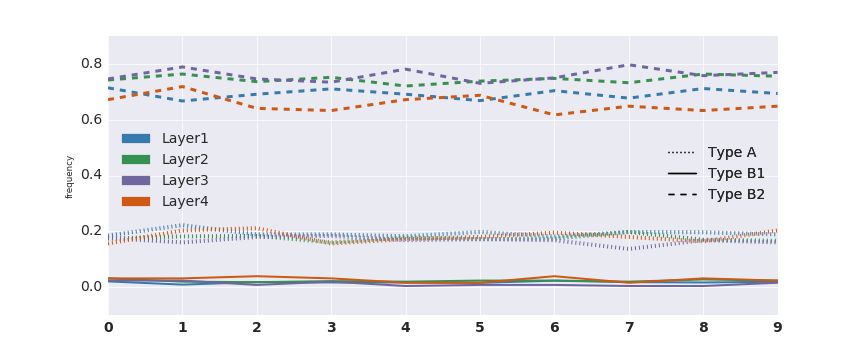
\includegraphics[width=1\linewidth]{neuron_types_across_digits.png}
    \captionof{figure}{\footnotesize{Frequencies of the three neuron types across layers and \newline digits. The line styles represent different neuron types; colors indicate \newline the four layers of the MLP. }}
    \label{fig:Neuron_types_digits_and_layers}
\end{minipage}
\hfill
\begin{minipage}{0.3\textwidth}
  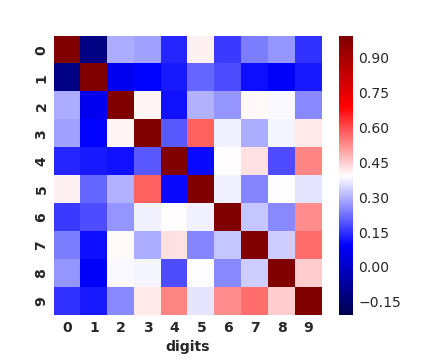
\includegraphics[width=1\linewidth]{corr_coeff_sn_lay4.png}
  \captionof{figure}{\footnotesize{Pearson correlation coefficients between Type A neurons in layer 4 for the ten digit-classes.}}
  \label{fig:TypeA_neurons_correlation}
\end{minipage}
% -------------------End Minipage-------------------------

%------------------------Begin Figure--------------------
\begin{wrapfigure}[13]{R}{0.5\textwidth}
\centering
  	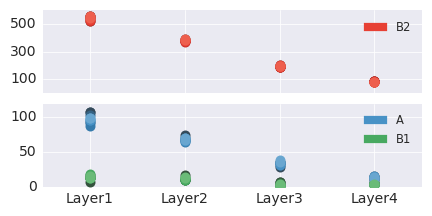
\includegraphics[width=\linewidth]{absolute_numbers.png}
  	\captionof{figure}{\footnotesize{Absolute number of neurons of each type per digit and layer.}}
    \label{fig:abs_numbers}
\end{wrapfigure}
%-----------------------End Figure-----------------------


\noindent Comparing the occurrence of the three neuron types across layers we find that for all three types the absolute numbers decrease as the layer numbers increase (see Figure \ref{fig:abs_numbers}). Considering that the total number of neurons per layer also decreases, this effect might be misleading. We therefore performed a more detailed analysis: first we split each dataset in $\mathcal{D}$ into subsets MNIST$_d^i$, with $i$ from $0$ to $9$ corresponding to the $10$ digit-classes ($\approx 1000$ samples each). For each sub-dataset and layer we then calculated the absolute amount of each of the three neuron types and finally normalized the results by the layer sizes. Figure \ref{fig:Neuron_types_digits_and_layers} shows that the percentage of each of the three types is stable, not only across layers but also across digits.\newline  

\noindent This might suggest, that even though these neurons play a role in classification, they are not themselves associated with individual digits. To test this hypothesis we compared the IDs of the type A neurons in layer 4 across all digit classes. Figure \ref{fig:TypeA_neurons_correlation} shows a heatmap of the resulting correlation coefficients where we see overall low correlation values. This suggests that the rotation sensitive Type A neurons are indeed tuned to specific digit types. \newline

\noindent Since we found that the occurrence of the three classes of neurons is not bound to a specific layer or digit, we will in the following limit our investigation to layer $4$ and digit $1$.

\section{Effect on classification accuracy}

\noindent First, we determine the neurons of each type by the procedure described above except that now we present the network only with samples depicting the digit  $1$ (i.e. MNIST$_d^1$). To find out how strongly the neurons of each type are tuned to recognize digit $1$, we use the unrotated sets MNIST$_0^i$ and compare how strongly the activity of each neuron type varies when presented with samples depicting different digits. The results are shown in the left column of Figure \ref{fig:Special_neurons_layer4 }. \newline

\noindent To characterize the neuron's impact on classification accuracy, we set the weights connecting them to the Softmax layer to 0, thereby ignoring their contribution to the classification procedure and effectively 'switching them off'. We then record the relative changes in accuracy by calculating for each digit $i$ and dataset $d$: 
	
\begin{displaymath}
\frac{a_w(MNIST_d^i) - a_{w^\prime}(MNIST_d^i)}{a_w(MNIST_d^i)}.
\end{displaymath}

\noindent Here $a_w(MNIST_d^i)$ means the classification accuracy of the unchanged network on the $MNIST_d^i$ dataset and $a_{w^\prime}$ means the accuracy of the altered network ($0$-weights from special neurons to Softmax). The relative changes in accuracy averaged over datasets are are shown in the right column of Figure \ref{fig:Special_neurons_layer4 }.\newline

%-------------------------- Begin Figure ---------------------
\begin{figure}
\centering
\begin{subfigure}{.7\textwidth}
  \centering
  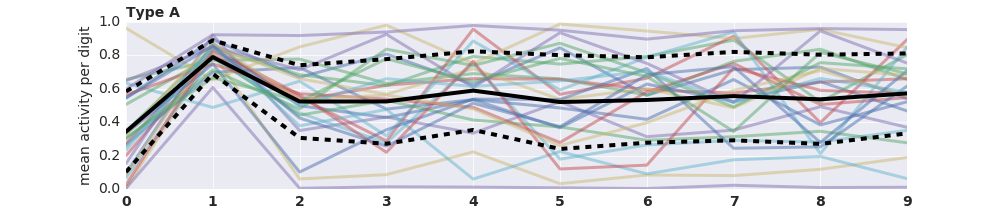
\includegraphics[width=1\linewidth]{activity_sn_digit1_lay4_mnist.png}
\end{subfigure}%
\begin{subfigure}{.3\textwidth}
  \centering
  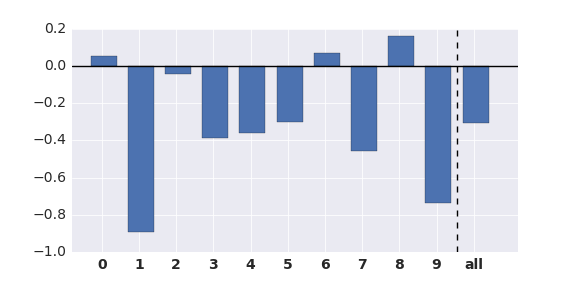
\includegraphics[width=1\linewidth]{rel_acc_dig1_lay4_typeA.png}
\end{subfigure}
\hfill

\centering
\begin{subfigure}{.7\textwidth}
  \centering
  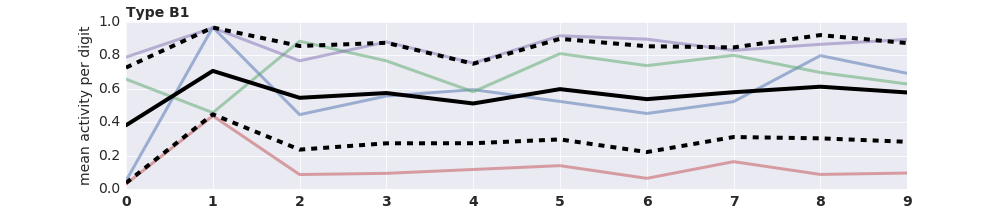
\includegraphics[width=1\linewidth]{activity_ih_digit1_lay4_mnist.png}
\end{subfigure}%
\begin{subfigure}{.3\textwidth}
  \centering
  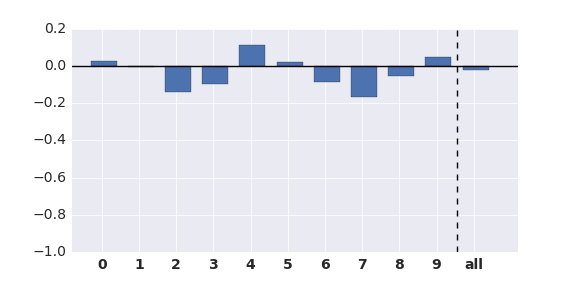
\includegraphics[width=1\linewidth]{rel_acc_dig1_lay4_typeB1.png}
\end{subfigure}

\hfill
 \centering
\begin{subfigure}{.7\textwidth}
  \centering
  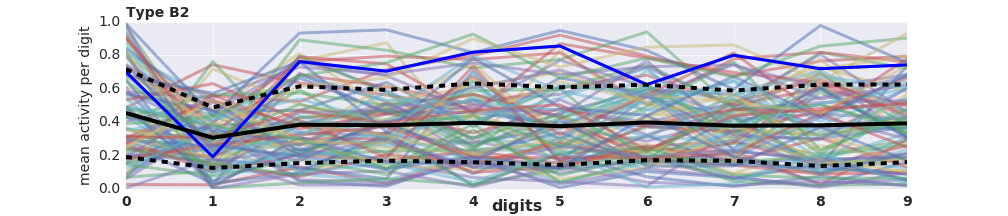
\includegraphics[width=1\linewidth]{activity_il_digit1_lay4_mnist.png}
\end{subfigure}%
\begin{subfigure}{.3\textwidth}
  \centering
  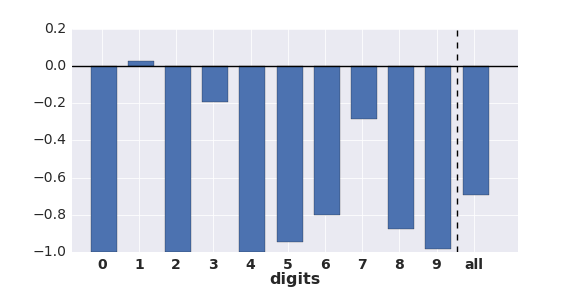
\includegraphics[width=1\linewidth]{rel_acc_dig1_lay4_typeB2.png}
\end{subfigure}
\caption{\footnotesize{The left column shows the mean activities of each type of neuron when presented with each digit-class. The right column shows the relative changes in accuracy when neurons of each type are switched off. Each row corresponds to one type of neuron: Type A in row 1, Type B1 in row 2 and Type B2 in row 3. All neurons were identified using the MNIST$_d^1$ sets depicting digit 1 in different degrees of rotation.}}
\label{fig:Special_neurons_layer4 }
\end{figure}
%-----------------------End Figure -----------------------------


\noindent The results for the 26 Type A neurons are shown in the first row of Figure \ref{fig:Special_neurons_layer4 }. On the left we see the mean activities of Type A neurons when presented with samples from the MNIST$_0^i$ sets. The thick black line shows the average over all Type A neurons, and the dotted lines indicate the standard deviations. It is clear that not only the mean activity is highest for MNIST$_{0}^{1}$ but also the variance has a minimum at this digit. This suggests that neurons of Type A are tuned to react to digit $1$. \newline

\noindent On the right side we see the relative changes in classification accuracy with respect to Type A neurons. Setting the weights of all connections from Type A neurons to the Softmax layer to 0 decreases the classification accuracy by almost 40\% (see rightmost bar). Looking at the results for individual digits, we see that for digit $1$ performance decreases drastically (almost 90\%). For other digits we find the decrease to be less strong, and sometimes we even see a slight increase. It is interesting that the decrease in performance is also strong for the digits 7 and 9, which share with digit 1 the property of a tilted straight line. \newline

\noindent For Type B neurons we observe quite different behavior. In row 2 we see that Type B1 neurons also show higher activity for the MNIST$_{0}^{1}$ dataset than for any other digit, but the classification accuracy for digit 1 is not affected by switching off these neurons. This might, however, be due to the fact that we only find 4 neurons of this type.\newline
\noindent  Type B2 (row 3) neurons on the other hand show decreased activity for the MNIST$_{0}^{1}$ dataset and slightly increased classification performance for digit one, whereas the accuracy for all other digits is strongly decreased. This might indicate that neurons of type B2 code for \textit{not 1}; i.e., they suppress the result $1$ whenever another digit is shown. This suggestion is affirmed also by the highlighted solid blue line in the activity plot, which gives an example of a neuron which is highly active for any digit \textit{but} 1.


%-------------------------Begin Figure------------------------
\begin{figure}[h]
\begin{center}
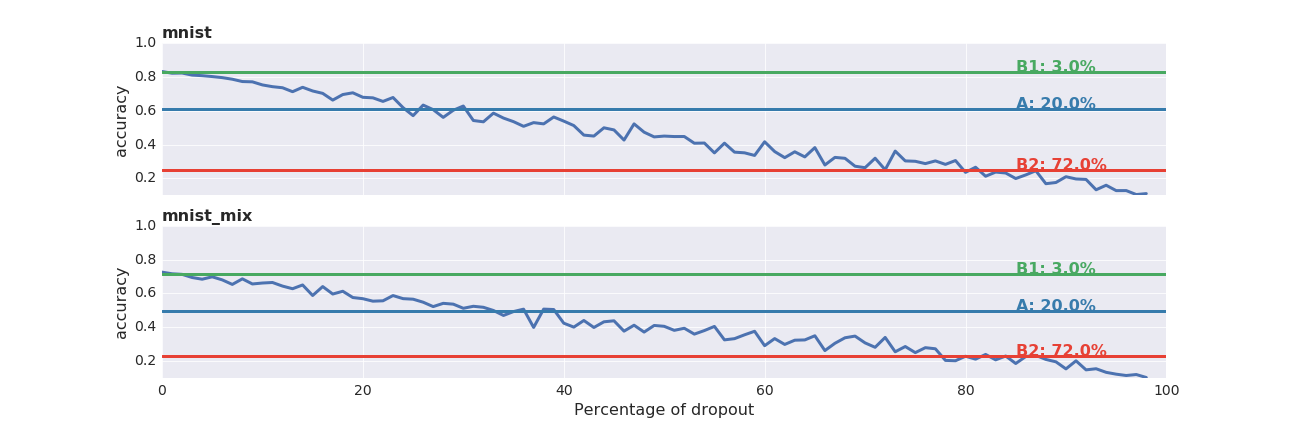
\includegraphics[scale = .4]{rand_vs_specific_dropout_lay4.png}
\caption{\footnotesize{The blue line shows the result of random dropout in layer 4. The x-axis indicates the percentage of dropped out neurons and the y-axis shows the resulting accuracy averaged over 10 trials each. The straight lines show the accuracy results after dropping out the neurons of Type A, B1 and B2 (for digit 1). The datasets used were MNIST$_0$ (upper plot) and MNIST$_{mix}$ (lower plot). }}
\label{droput}
\end{center}
\end{figure}
%-------------------------End Figure------------------------


\noindent In Figure \ref{droput} we compare the effect of the dropout of special neurons to the dropout of randomly selected neurons. The straight lines indicate the accuracy after the dropout of each of the three neuron types. We can see that neurons of type A most strongly affect the classification accuracy, because even though they make up only 20\% of the neurons in layer 4, they affect the accuracy as much as the dropout of nearly twice as many randomly chosen neurons (both for MNIST$_0$ and MNIST$_{mix}$). 
\newpage
\section{Discussion}
In this project we initialized a MLP with parameters from an AE trained to reconstruct rotated images of the MNIST dataset. The aim was to study whether the network would arrive at a rotation-invariant representation of the inputs and in which way information about the rotation would be conserved. \newline
\noindent We found that using the parameters from the AER autoencoder allowed for much more reliable classification of rotated digits. Also, as the input passes through the layers of the MLP, resulting activations become less affected by different degrees of rotation (see Figure \ref{fig:Euclidian_distances}).  
However, we also found that throughout all layers the neurons which play an important role in classification (i.e. those which have a high chance of being among the most active ones) do show sensitivity to rotation. This means that the network does not arrive at completely rotation-invariant representations of the digits. 


 \begin{thebibliography}{5}

	\bibitem{Olshausen}
	BA.~Olshausen et al.: "A neurobiological model of visual attention and invariant pattern recognition based on dynamic routing of information." {\em  Journal of Neuroscience},
	vol.~13, no.~11, pp.~4700-4719., Nov. 1993.

	\bibitem{Benigo}
	Y.~Bengio et al.: "Greedy Layer-Wise Training of Deep Networks." In {\em Advances in Neural Information Processing Systems 19 }, ed. B. Schölkopf et. al MIT Press, 2007, pp. 153 -160

	\bibitem{Oliver}
	O.~Eberle: "Investigating visual invariance in object classification using deep denoising autoencoders" {\em Lab Rotation Report }, supervision Prof. Klaus Obermayer, Youssef Kashef
 
\end{thebibliography}
%
%
%
%\newpage 
%\section*{Appendix}
\begin{flushleft}
\begin{figure}[h]
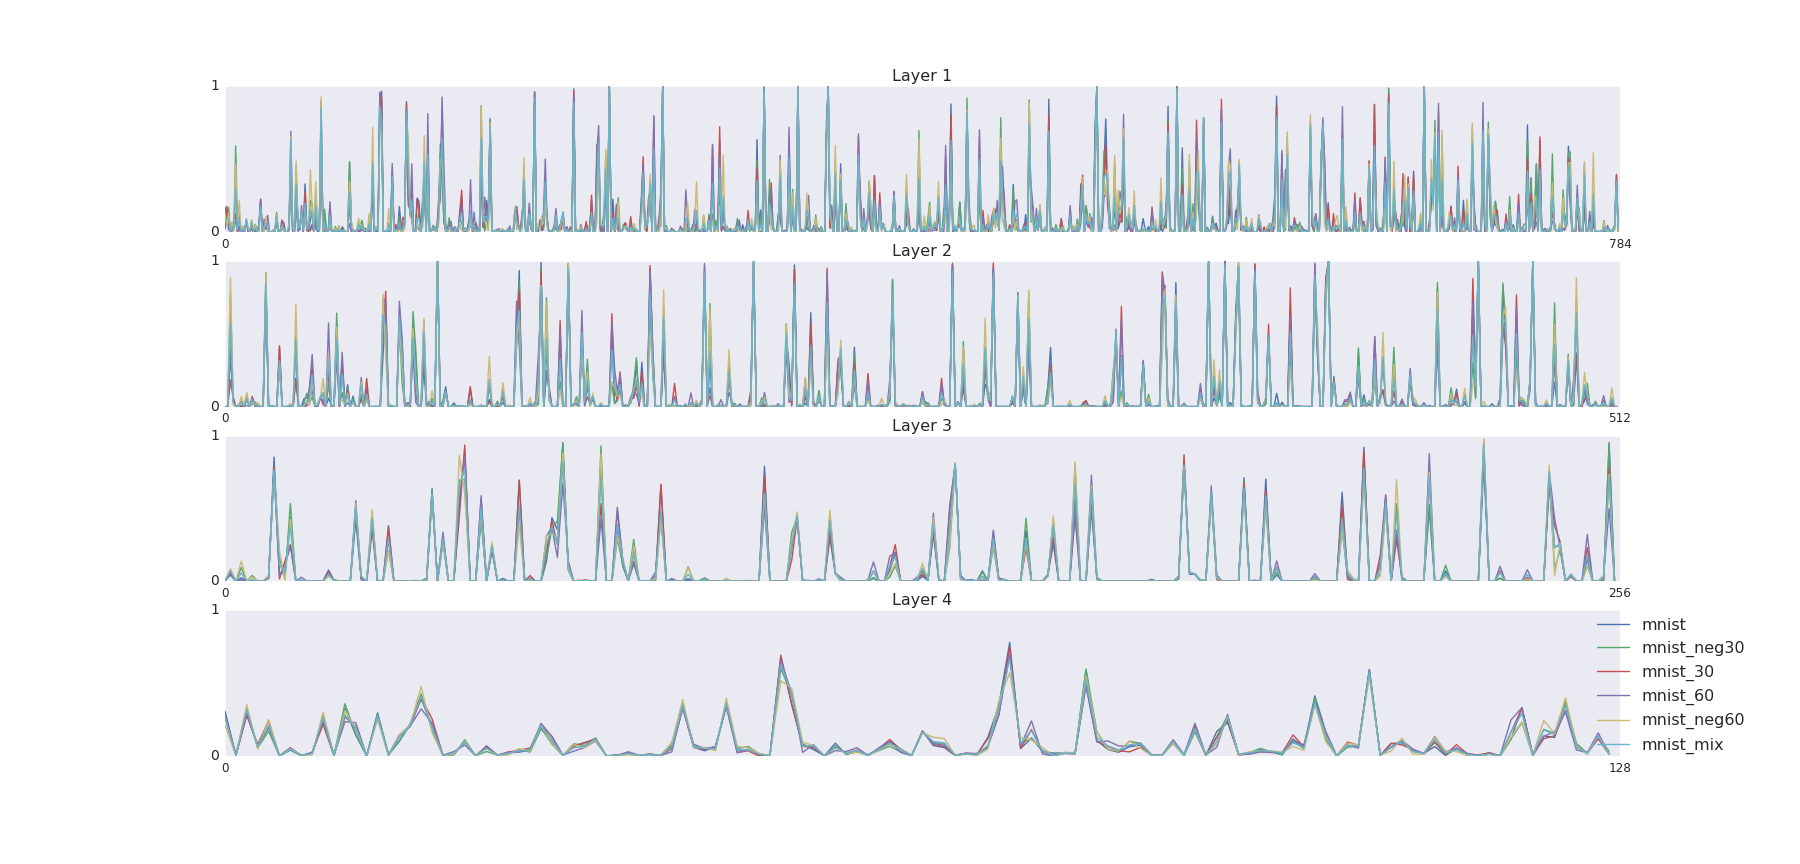
\includegraphics[angle=90,origin=c, scale = .35]{most_active_neurons_6datasets.png}
%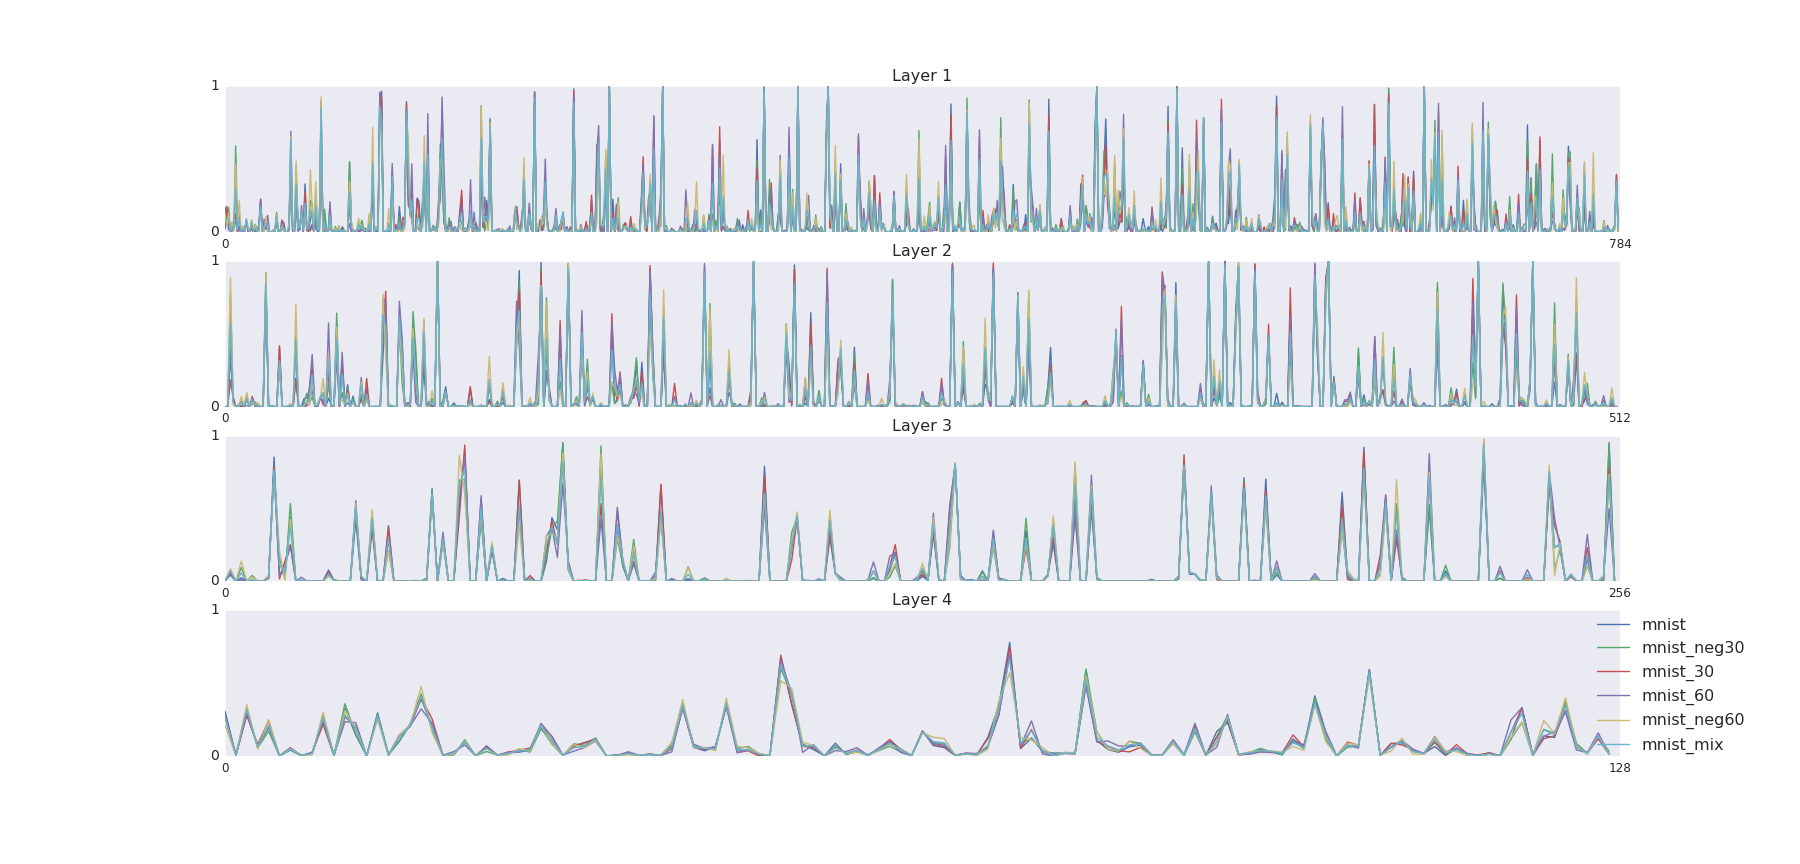
\includegraphics[scale =.3]{most_active_neurons_6datasets.png}
\caption{\footnotesize{Values of $p_{10}(n)$ for all four layers and the six datasets in $\mathcal{D}$ Layers are displayed from top (layer 1) to bottom (layer 4). Also note the differences in x-axis due to decreasing layer size.}}
\label{fig:MostActive_all}
\end{figure}
\end{flushleft}




% \begin{figure}[b!]
% 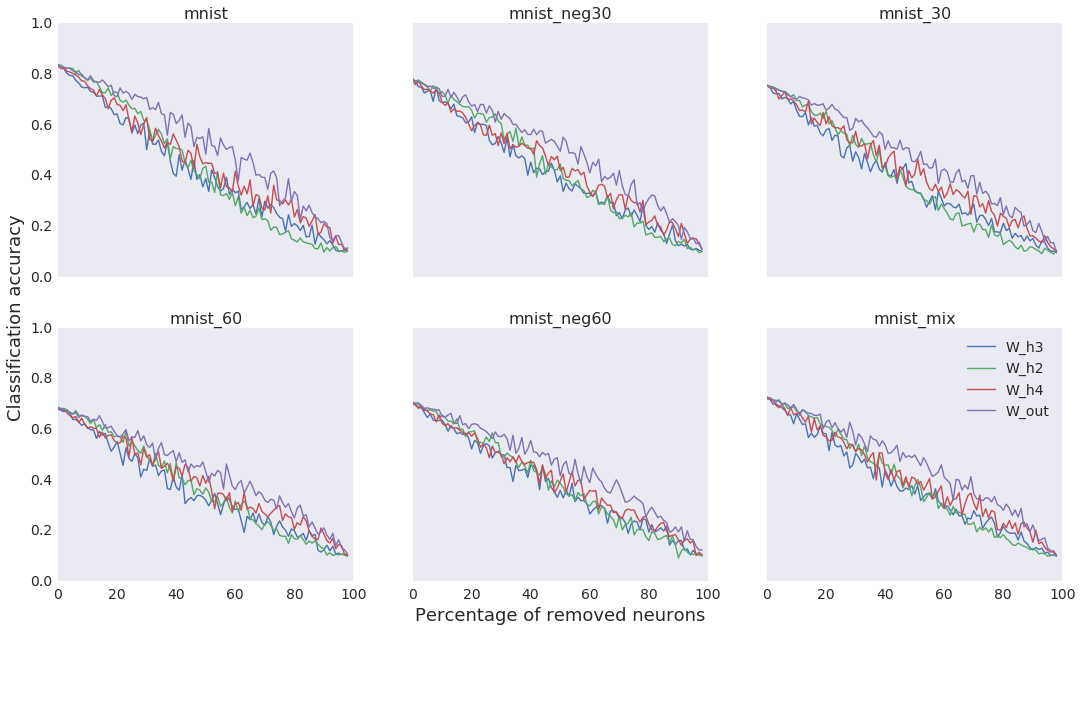
\includegraphics[width=1\textwidth]{Compare_dropout_layerwise.png}
% \caption{\footnotesize{blaj}}
% \label{fig:Dropout}
% \end{figure}

% show that the scaling neurons in layer 4 differ across digits! 


\end{document}
